%!TEX TS-program = xelatex
% vim: set fenc=utf-8

% -*- coding: UTF-8; -*-
%!TEX encoding = UTF-8
\documentclass[twoside]{CUGThesis}

\RequirePackage{setspace}
%设置命令
\newcommand{\makestatement}[2][0]{
	\clearpage
	\thispagestyle{empty}
	\vspace*{1em}
	\begin{center}
\begin{spacing}{1.25}{
		\hei \sanhao
		学士学位论文原创性声明
}
\end{spacing}
	\end{center}


\begin{spacing}{1.1}
 \song \xiaosihao

本人郑重声明:所呈交的学位论文是本人在导师指导下独立进行研究工作所取得的研究成果。
除了文中特别加以标注引用的内容外,本论文不包含任何其他个人或集体已经
发表或撰写的成果作品。本人完全意识到本声明的法律后果由本人承担。\\
\end{spacing}

	\begin{spacing}{1}
	\rightline{
	\begin{tabular}{r}
		\\
		作者签名:\hspace{10em}
		 \hspace{4em}年 \hspace{2em} 月 \hspace{2em} 日
	\end{tabular}
	}
	\end{spacing}

	\vspace*{3em}

	\begin{center}
	\begin{spacing}{1.25}{
		\hei \sanhao
		学位论文使用授权书
	}
	\end{spacing}
	\end{center}

\begin{spacing}{1.1}
\song \xiaosihao

本学位论文作者完全了解学校有关保障、使用学位论文的规定,同意学校保留并向有关学位论文管理部门或机构送交论文的复印件和电子版,
允许论文被查阅和借阅。本人授权省级优秀学士学位论文评选机构将本学位论文的全部或部分内容编入有关数据库进行检索,
可以采用影印、缩印或扫描等复制手段保存和汇编本学位论文。\\
\end{spacing}
本学位论文属于
	\begin{enumerate}
		\item 保密 $\Box$,在\uline{\makebox[3em]}年解密后适用本授权书。
		\item 不保密 $\Box$。
	\end{enumerate}
	(请在以上相应方框内打``$\surd$'')

	\begin{spacing}{1}
		\rightline{
		\begin{tabular}{r}
			\\ \\ 
			作者签名:\hspace{10em}
			 \hspace{4em}年 \hspace{2em} 月 \hspace{2em} 日
			 \\ \\  
			 导师签名:\hspace{10em}
			 \hspace{4em}年 \hspace{2em} 月 \hspace{2em} 日
		\end{tabular}
		}
		\end{spacing}
	\vspace{4em}
	\clearpage
}

\include{title}

\title{基于IPv6的HTTP/2过渡应用的设计与实现} %论文题目
\author{陈立翔} %作者姓名
\date{\today} %日期,默认当日
\school{计算机学院} %院系名称
\classnum{计算机科学与技术} %专业
\stunum {20151001270} %学号
\instructorone{张峰} %指导教师1姓名
\instructoronelevel{副教授}
\instructortwo{陈伟涛} %指导教师2姓名
\instructortwolevel{副教授}

\usepackage{makecell}
\usepackage{multicol}
\usepackage{multirow}
\usepackage{hyperref}

\begin{document}
	\maketitle
	\makestatement

	\begin{cnabstract}{IPv6 协议;HTTP/2协议;HTTP 网关;反向代理;负载均衡;Go语言;}
		今天,网络早已成为人们生活中不可缺少的部分。同时随着我国网民人口的不断增长,
	互联网环境正在变得愈发复杂。在服务端,开发和运维人员需要利用有限的服务器资源应对更大的并发请求和越来越多的潜在的网络攻击。
	在这种情况下,原有的一些网络协议已经无法满足要求。目前,IPv4的公网地址资源已经枯竭,早在2011年
	亚洲地区就已经无法分配到IPv4地址;而HTTP/1.x协议经过若干次修订后依然被诟病效率过低和功能不足。
	RFC 发布的 IPv6和HTTP/2协议相关标准已经在很大程度上解决了这些问题,
	如何将旧有的Web应用过渡支持IPv6和HTTP/2是我们目前面临的重要挑战。\par
		本文对于如何让现有的IPv4环境下仅支持HTTP/1.x协议的Web应用能够在IPv4和IPv6双栈环境下工作并
	支持HTTP/2协议,同时尽可能提高服务端的并发性能,开展了以下研究工作:
	\begin{enumerate}
		\item 通过对 Go 语言技术的深入研究,分析其协程和并发模型的技术特点。Go 语言是一门在语言层面
		实现了协程的语言,其实现能够避免操作系统调用产生的开销,单机轻松构建百万级协程,CPU资源的利用率极高,
		是近年来服务端开发中解决高并发问题的重要突破点。
		\item 比较了 RFC 标准中 HTTP/1.x 和 HTTP/2 报文的区别,分析了如何将 HTTP/1.x 的报文加工处理
		成 HTTP/2 的报文。同时结合 Go 语言中原生的 net/http 和 tls 库对报文增加 HTTPS 加密,从而
		兼容目前主流浏览器的实现。
		\item 为了将 HTTP/1.x 应用过渡支持 HTTP/2 ,本文采用 Go 语言技术设计了一个 HTTP 网关。该网关
		通过反向代理技术,在无需对原有应用进行任何修改的情况下,将其升级为支持 HTTP/2 协议,并可在 IPv4和
		IPv6双栈环境下工作。
		\item 基于加权轮询算法和一致性哈希算法对该网关设计了负载均衡策略,
		使得该网关能够支持横向扩容的 Web 应用,应对更复杂的并发情况。
		\item 对该网关进行了压力测试,对比目前市场上提供反向代理功能的服务器如 Apache, Nginx 等,
		得出该网关在一些情况下能够提高系统并发数和减少响应时间,提升用户体验。并通过火焰图分析该网关在
		实际工作环境中的性能瓶颈。
	\end{enumerate}
		\par
		综上所述,本文设计的基于 Go 语言的 HTTP 反向代理网关,能够作为在IPv4和IPv6双栈环境下的 HTTP/2 过渡应用,
	并且具有较好的并发性能。经过测试,具有一定实用价值。
	\end{cnabstract}
	
	% \begin{enabstract}{keyword; keyword; keyword; keyword}
	% 	abstract
	% \end{enabstract}
	
	\makeToc
	
	%---------------------------------------------开始正文---------------------------------------------
	
	%--------------------------------------------- 第一章 ---------------------------------------------
	\begin{spacing}{2}
		\section{绪论}
	\end{spacing}
	\subsection{研究背景及其意义}
	各种网络协议常常被称为互联网时代的基石。随着网络环境的变化,网络协议也需要适应时代的需求
	迭代升级。\par
	从1996年开始,一系列关于IPv6协议的RFC标准发表出来,旨在取代原有的IPv4协议。IPv6的地址长度为
	128位,能提供远多于IPv4 的地址数量。在IPv6环境下,将不需要IPv4环境下为了解决地址数量不足而衍生出的NAT等技术,每个设备都能得到
	一个公网IP,有利于物联网等技术的发展。但IPv6技术的推进还需要一段时间,在未来一段时间内我们都将
	面临着IPv4和IPv6共存的互联网环境。\par
		2015年发布的HTTP/2协议则旨在取代HTTP/1.x协议。为了提高网络传输的效率,更有效地利用网络资源,
	该协议增加了二进制分帧,多路复用和头部压缩等新的特性。同时目前浏览器中 HTTP/2 
	实现都强制要求数据通过 HTTPS 加密,而不是像 HTTP/1.x 协议那样
	将数据明文发送。这显著增强了数据传输的安全性,有效避免数据被劫持等安全隐患。\par
	将现有的应用迁移升级到这些新协议上将会是一个漫长且耗资巨大的过程。如何在今天这种多种协议共存的情况下,
	将旧有的应用以尽可能低的成本过渡迁移到新协议上,且具有较好的性能?\par
		目前国内外最广泛使用的HTTP服务器Apache和Nginx都支持反向代理并升级IPv6和HTTP/2协议的功能。
		通过配置都可以支持通过反向代理将旧有的服务升级至支持IPv6和HTTP/2协议。

	\subsection{国内外相关工作介绍}
	目前国内外市场上90\%以上的反向代理HTTP网关服务器为Apache 和 Nginx。这两者都基于C语言编写。也有很多人对这些网关进行了二次开发,例如中国工程师章亦春等人基于Nginx开发的OpenResty\cite{OpenResty}等。\par
	这些网关在不断的迭代过程中也陆续加入了IPv6和HTTP/2协议的支持。它们由于久经实际生产环境考验,具有较强的稳定性。
	但由于一些历史遗留原因,也或多或少存在诸如开发效率较低,并发能力较差等问题。
	\subsubsection{Apache}
	Apache HTTP Server (简称Apache)是 Apache 软件基金会维护开发的一个开源HTTP服务器软件。它自1995年诞生以来,
	一直是世界上最被广泛使用的HTTP Server。同时其也提供反向代理功能,并已加入 HTTP/2 和 IPv6 的支持。\par 
	Apache在二十多年间已迭代数个版本,具有极佳的稳定性和大量的插件,能够帮助开发者快速构建小型Web应用。\par
	但是 Apache 在应对并发请求时,使用的是传统上基于进程或线程模型架构,通过多线程来处理并发请求。
	事实上这种模型虽然稳定,却无法发挥出现代计算机的性能,后面在讨论Go语言的并发模型时将会谈到这一点。\par
	\subsubsection{Nginx}
	Nginx是俄罗斯工程师Igor Sysoev在2004年发布的一款异步框架的高性能HTTP服务器,常被用作反向代理和负载均衡器。
	目前绝大多数高并发量的网站都使用Nginx作为HTTP服务器。它在不断的迭代中也陆续加入了IPv6和HTTP/2的支持。\par
	Nginx的出现就是为了解决Apache的并发模型无法解决的C10K问题。C10K指的是能够使单机服务器承受一万以上的并发连接请求。
	Nginx创造性地将模块化加入了设计之中,非常方便于二次开发。如由中国工程师章亦春等人开发的OpenResty,
	阿里巴巴公司开发的Tengine都是根据实际需求基于Nginx二次开发的HTTP服务器。\par
	Nginx采用了epoll多路复用机制来应对高并发请求。epoll是Linux 2.6版本内核之后加入的特性。
	Linux提供了三种I/O多路复用模型,select, poll 和 epoll。它们分别是基于数组,链表和哈希表保存文件描述符的
	I/O多路复用模型。显然2.6版本加入的epoll模型所使用的哈希表具有最低的时间复杂度,
	这可以大大减少操作系统切换上下文的开销,应对高并发连接。根据官方的测试结果,在理想情况下,Nginx单机
	可以应对五万个并发连接,而在实际的运作中,可以支持二万至四万个连接。\par 
	但是这也给Nginx带来了一个问题.在非Linux系统下,无法使用这些操作系统底层的API来进行I/O多路复用,这时
	其并发性能会大大下降。对于情况较为复杂的跨平台服务端解决方案来说,Nginx并不合适。\par
	\subsection{论文主要工作和章节结构}
	本文主要针对如何在IPv4和IPv6双栈环境下将旧有的HTTP/1.x的Web服务过渡升级支持HTTP/2设计了一个
	网关。该网关通过反向代理的形式升级协议。并且该网关具有高并发和易跨平台的特性,避免了上述解决方案的一些缺点。\par 
	论文的内容和章节结构如下:
	\begin{enumerate}
		\item 第一章:绪论。主要介绍了研究背景,以及通过反向代理升级IPv6和HTTP/2协议的这方面国内外的
		一些成熟解决方案及其存在的问题,以及本文主要工作安排。
		\item 第二章:Go 语言服务端相关技术介绍。简单介绍了Go语言的背景和一些内置库实现,并分析了其并发模型,
		说明了Go语言应用在本项目的一些优势。
		\item 第三章:HTTP/1.x 到 HTTP/2 的转换实现。深入分析了RFC标准中 HTTP/1.x 协议和 HTTP/2 协议的
		差异,根据这些差异拟定了程序中通过怎样的流程去升级HTTP协议。同时也对广泛使用的Websocket协议做了处理。
		\item 第四章:IPv4 和 IPv6 双栈环境下反向代理功能的实现。
		\item 第五章:性能测试。
	\end{enumerate}
	
	%------------------------------------------- 第二章 ---------------------------------------------
	\begin{spacing}{2}
		\section{Go语言相关技术介绍}
	\end{spacing}
	\subsection{Go语言简介}
	Go语言(简称Go)是由美国谷歌(Google)公司发布的一种静态强类型、编译型、并发型并具有垃圾回收功能的编程语言,于2009年推出最初版本并开源。
	其作者 Rob Pike 和 Ken Thompson 等人均曾经在美国贝尔实验室工作,参与了C语言和Unix系统的开发工作。\par 
	Go的发明是为了解决C++在服务端开发时的一些问题。在高并发环境下,C++由于其过多的语言特性,导致编写并发程序较为复杂。
	同时其较为落后的包管理机制不利于对代码的高效复用。依赖于系统底层API的网络操作等也使得其跨平台能力不强。\par
	Go本身语法十分接近C语言,甚至比C语言还要更简单一些,其关键字数量比C语言还要更少。对于有一定C语言开发经验的开发者来说学习成本较低。
	Go内置大量网络编程相关的库,可以大大简化网络编程的工作,更重要的是,其实现不依赖于任何操作系统底层API,
	这使得Go编写的程序可以较为容易地交叉编译并在多平台运行。\par
	Go程序以包的形式组织。包实质上是一个包含Go文件的文件夹。包内的代码共享相同的命名空间,为区分包内
	包外的私有成员,Go将以大写字母开头的对象(包括函数,变量等)对其它包可见,其它的则不可见。\par 
	\subsection{Go语言的并发模型}
	Go语言最为重要的特性来源于其在语言层面对并发的支持。这里讨论的是 Go 1.7 版本及之前的经典并发模型。
	虽然在后期版本增加了一些新的功能或语法糖,但本质上还是离不开我们后面讨论的这些并发模型。
	\subsubsection{协程(Coroutine)}
	我们知道,线程和进程都是在操作系统层面上实现的。相对于进程来说,线程可以减少调用时的上下文开销,具有更小的颗粒度。\par 

	\subsubsection{通道(Channel)}
	\subsubsection{上下文(Context)}
	
	
	
	%--------------------------------------------- 第三章 ---------------------------------------------
	\begin{spacing}{2}
		\section{HTTP/1.x到HTTP/2的转换实现}
	\end{spacing}
	要想实现HTTP/1.1到HTTP/2的转换,我们首先要了解这两个协议的特性及其异同,针对性地设计转换的方法。\par
	世界上最早的HTTP协议标准源于1991年发布的HTTP/0.9标准。该版本及其简单,只有一个HTTP方法 GET。它具有
	以下特点:
	\begin{itemize}
		\item 客户端/服务端响应都是ASCII字符
		\item 客户端请求由一个回车符(CRLF)结尾
		\item 服务器响应的是超文本标记语言(HTML)
		\item TCP连接在文档传输完毕后断开
	\end{itemize}
	\par
	显然这个协议是十分简陋的。它无法处理用户登录等稍微复杂一点的操作,以及各种富文本。1996年RFC发布了正式的HTTP/1.0标准,
	相较于之前的版本它有一些明显的特性:
	\begin{itemize}
		\item 服务端响应增加了响应状态
		\item 请求和响应增加了多行首部
		\item 响应内容不再局限于HTML
	\end{itemize}
	\par
	HTTP/1.0依然存在很多问题和值得优化的地方。比如对TCP连接的复用,大文件传输的优化,浏览器缓存较差等等。
	1999年发布的HTTP/1.1就是为了解决这些问题的。该协议一直到2014年,依然在不断地进行修订。它具有以下
	几个显著特性:
	\begin{itemize}
		\item 持久连接(Keep-Alive机制)
		\item 传输编码(Chunk机制)
		\item 字节范围请求(Accept-Ranges)
		\item 增强的缓存机制(协商缓存和强缓存)
	\end{itemize}
	\par
	HTTP/1.1已经有二十年的历史,并且依然在被广泛使用,十分稳定。但2015年,RFC依然发布了HTTP/2用于取代
	HTTP/1.1。这源于互联网快速的发展,使得其无法适应当前的需求。\par 

	\subsection{HTTP/1.1的困境}
	如今的Web应用已经大大超出了人们在最开始对Web的想像。在早期,一个网站往往只有一个简单的HTML页面。
	但是在今天,任意一个门户网站都有大量的流媒体,AJAX请求,图片……人们也不再仅仅使用PC来浏览网页,
	移动端和物联网设备逐渐成为了主流。这种情况下,一个Web页面中的HTTP请求数和网站所占用的通信和存储空间会大大增加。
	httparchive.org对目前互联网的的大量网站做了监测,结果如图所示\cite{httparchive}。\\ 
	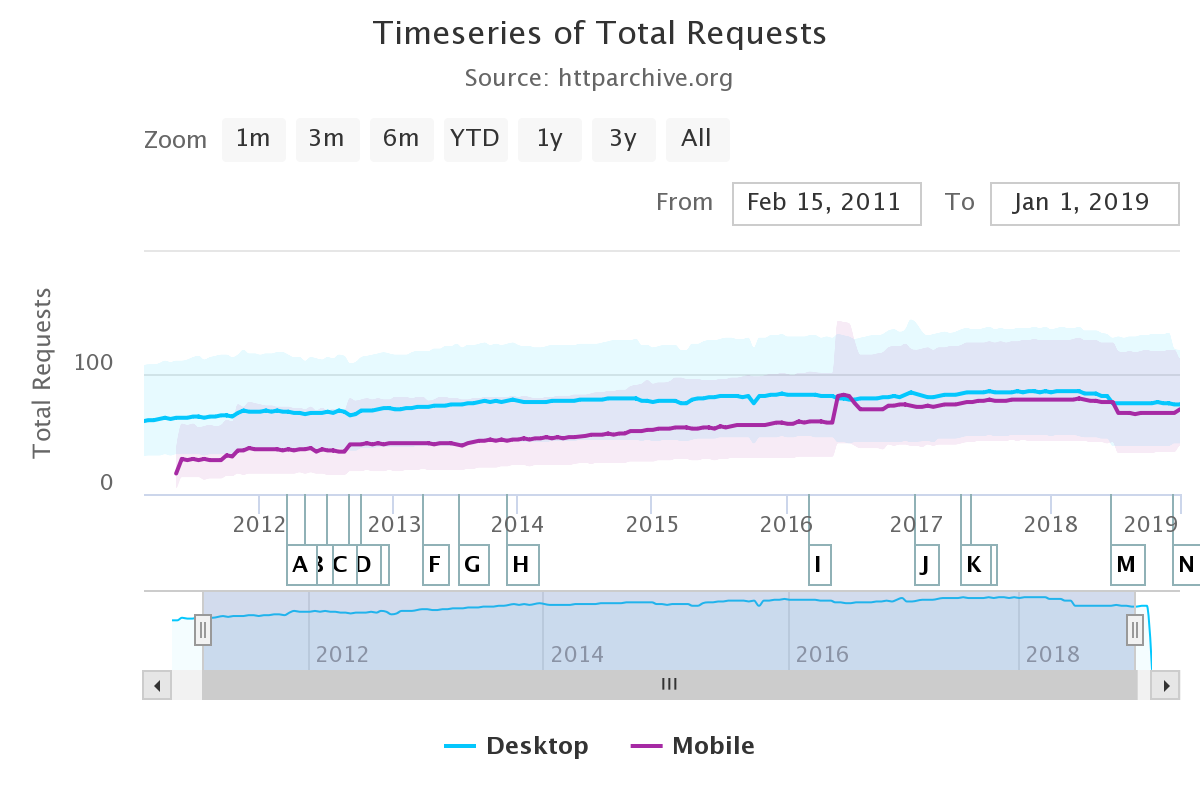
\includegraphics[scale=0.31]{Figures/web_total_reqs.png}\\
	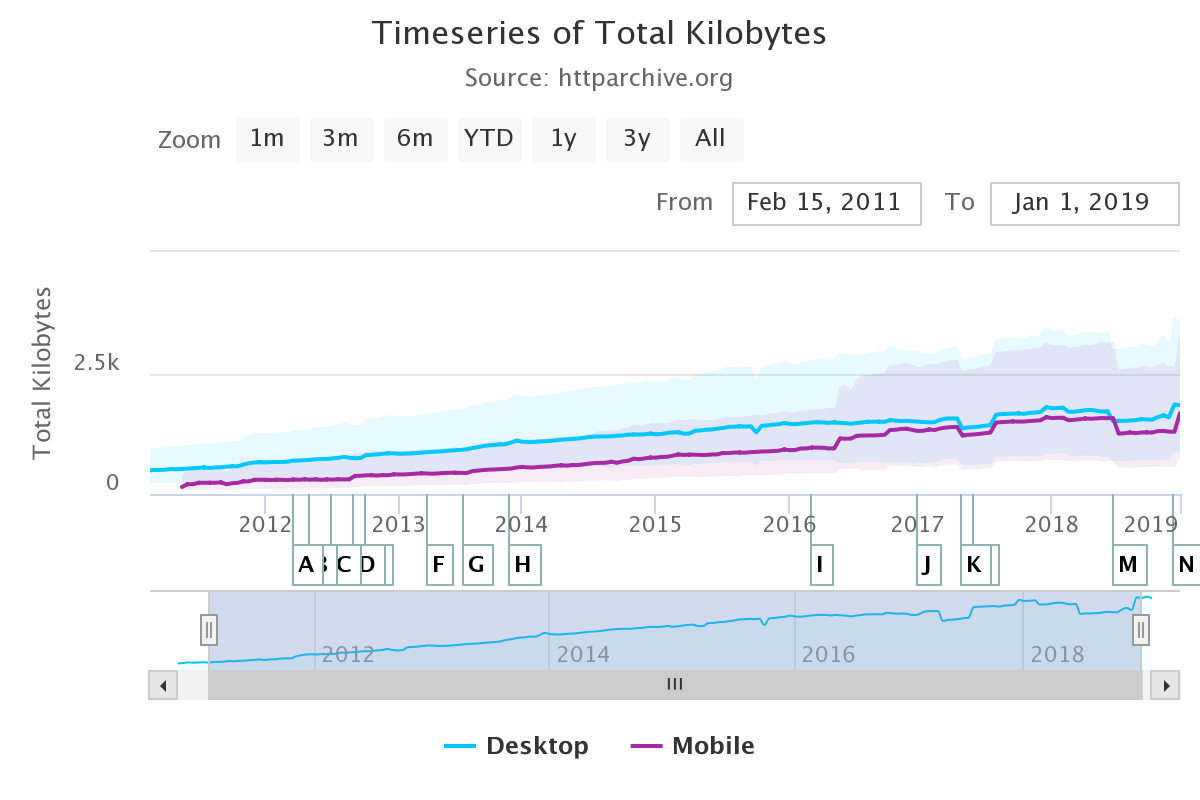
\includegraphics[scale=0.31]{Figures/web_total_size.png}\\
	\par 
	从图中可以看出,随着时间的推移,浏览一个网站平均需要的HTTP请求数量和资源的大小都在稳步上升。
	目前在没有缓存的情况下,在PC端浏览每个网站平均需要下载2000kb以上的资源,发生70个以上的HTTP请求。在
	移动端这个数字还要更高。这给了网络传输以很大的挑战。事实上,
	用户浏览网站时,在等待的过程中,平均有69.5\%的时间是耗费在网络操作的阻塞上的。\par 
	而HTTP/1.1协议本身对并发连接并没有做很好的优化。Keep-Alive机制本身只能复用连接,但是对并发连接并没有什么帮助。
	早期的标准RFC2616甚至规定浏览器中同域名只能有两个连接。
	RFC7230虽然去掉了这一限制,但现代浏览器中依然限制同域最多只能有6个并发连接。在浏览器中打开一个HTTP/1.1的网站,
	我们很容易在控制台中看到网络资源的加载时序,如图所示。\\ \par 
	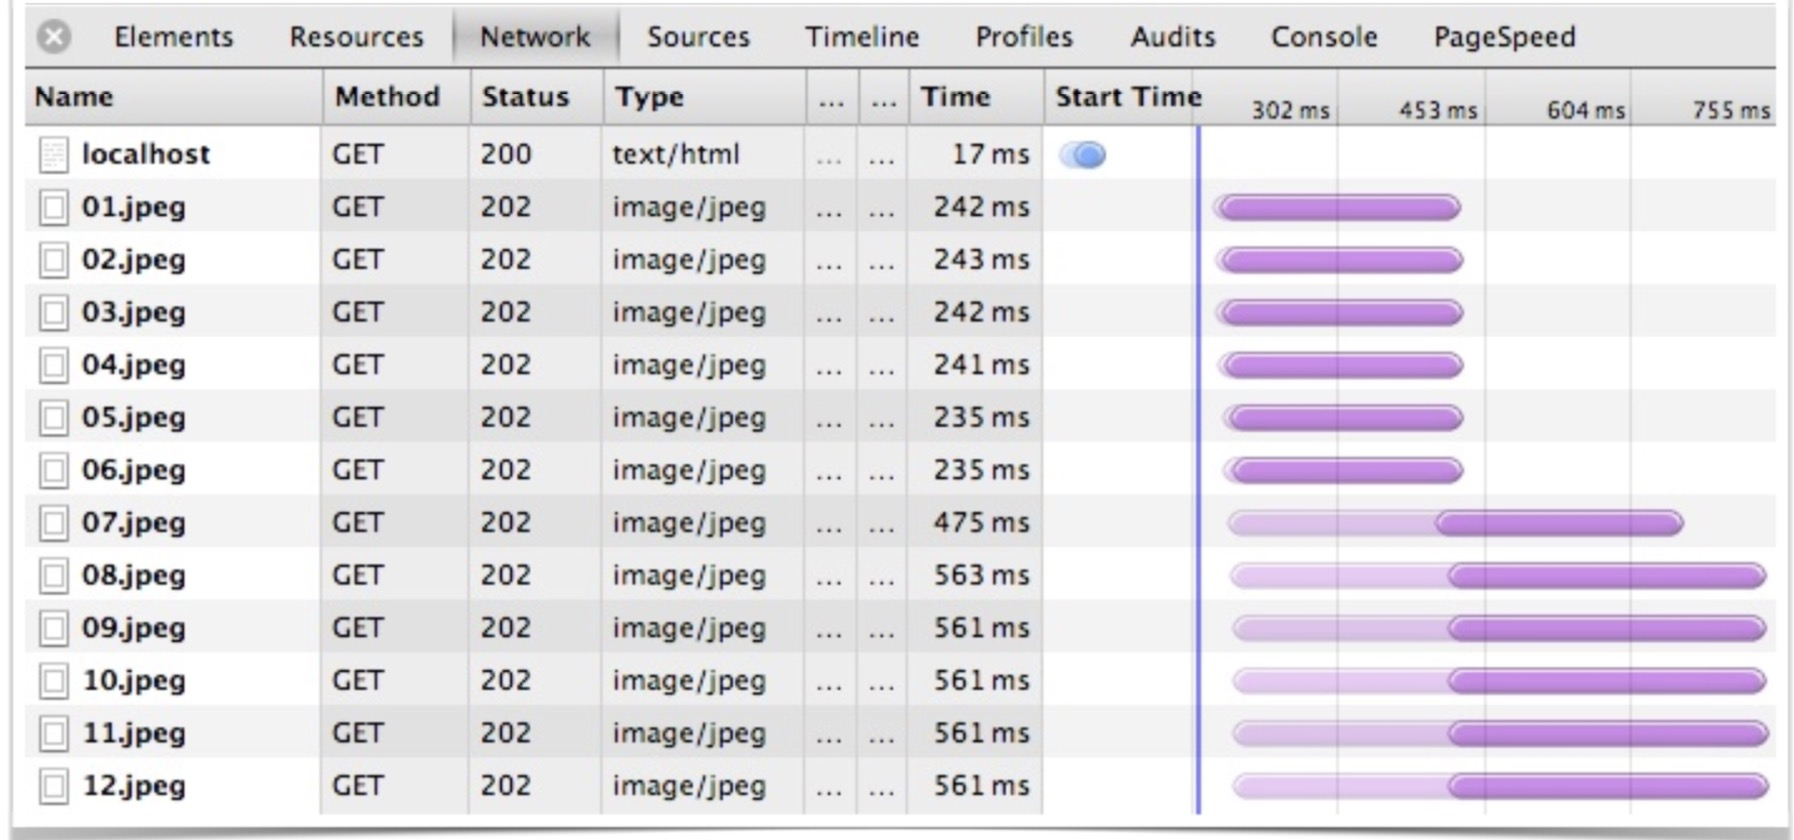
\includegraphics[scale=0.2]{Figures/web_load.jpg}
	\subsection{HTTP/2的新增特性}
	针对上文提到的HTTP/1.1的问题,2015年RFC发布的HTTP/2协议新增了若干特性:
	\begin{itemize}
		\item 引入了流(Stream)的概念,取消了Keep-Alive而采用多路复用机制。
		\item 引入二进制分帧,将消息分割为更小的帧,并采用二进制格式进行编码。其中头(Header)会被专门封装到Headers帧中。
		\item 引入头部压缩机制,将一些常用头部用单字节表示,缩减头部大小。
	\end{itemize} \par
	这些机制解决了并发连接的问题,并在一定程度上缩减了每次HTTP传输的大小。\par 
	特别需要注意的是,HTTP/2目前有H2C和H2两种实现类型。H2C是目前主流浏览器所实现的类型,
	该实现较为强调传输的安全性,强制通过TLS加密传输的数据。
	H2多用于非Web的应用场景,例如RPC调用等。下文所讨论的均默认为H2C的实现。
	\subsection{HTTP/2协商机制}
	在HTTP/1.1和HTTP/2共存的环境下,浏览器和客户端要怎么样才能知道到底应该选择哪个协议来沟通?
	毕竟还有很多低版本浏览器不支持HTTP/2。
	\subsection{WebSocket支持}

	\subsection{HTTPS支持}

	

	%-- 第四章
	\begin{spacing}{2}
		\section{IPv4和IPv6双栈环境下反向代理功能的实现}
	\end{spacing}
	\subsection{用户配置}
	\subsection{反向代理的实现}
	\subsection{负载均衡策略}
	\subsubsection{加权轮询算法(Weighted Round Robin)}
	\subsubsection{一致性哈希算法(Consistenting Hashing)}
	\subsection{IPv6环境下工作}

	%-- 第五章
	\begin{spacing}{2}
		\section{性能测试}
	\end{spacing}
	\subsection{压力测试}

	\subsection{火焰图}
	
	
	%---------------------------------------------  致谢  ---------------------------------------------
	\begin{spacing}{2}
		\section*{致谢}
	\end{spacing}
	\phantomsection
	\addcontentsline{toc}{section}{致谢}
	
	致谢
	
	\clearpage
	%---------------------------------------------参考文献---------------------------------------------
	
	\bibliography{Bibs/mybib}
	\phantomsection
	\addcontentsline{toc}{section}{参考文献}
	
\end{document}